\chapter{Visualization}

\begin{figure}[h]
  \centering
  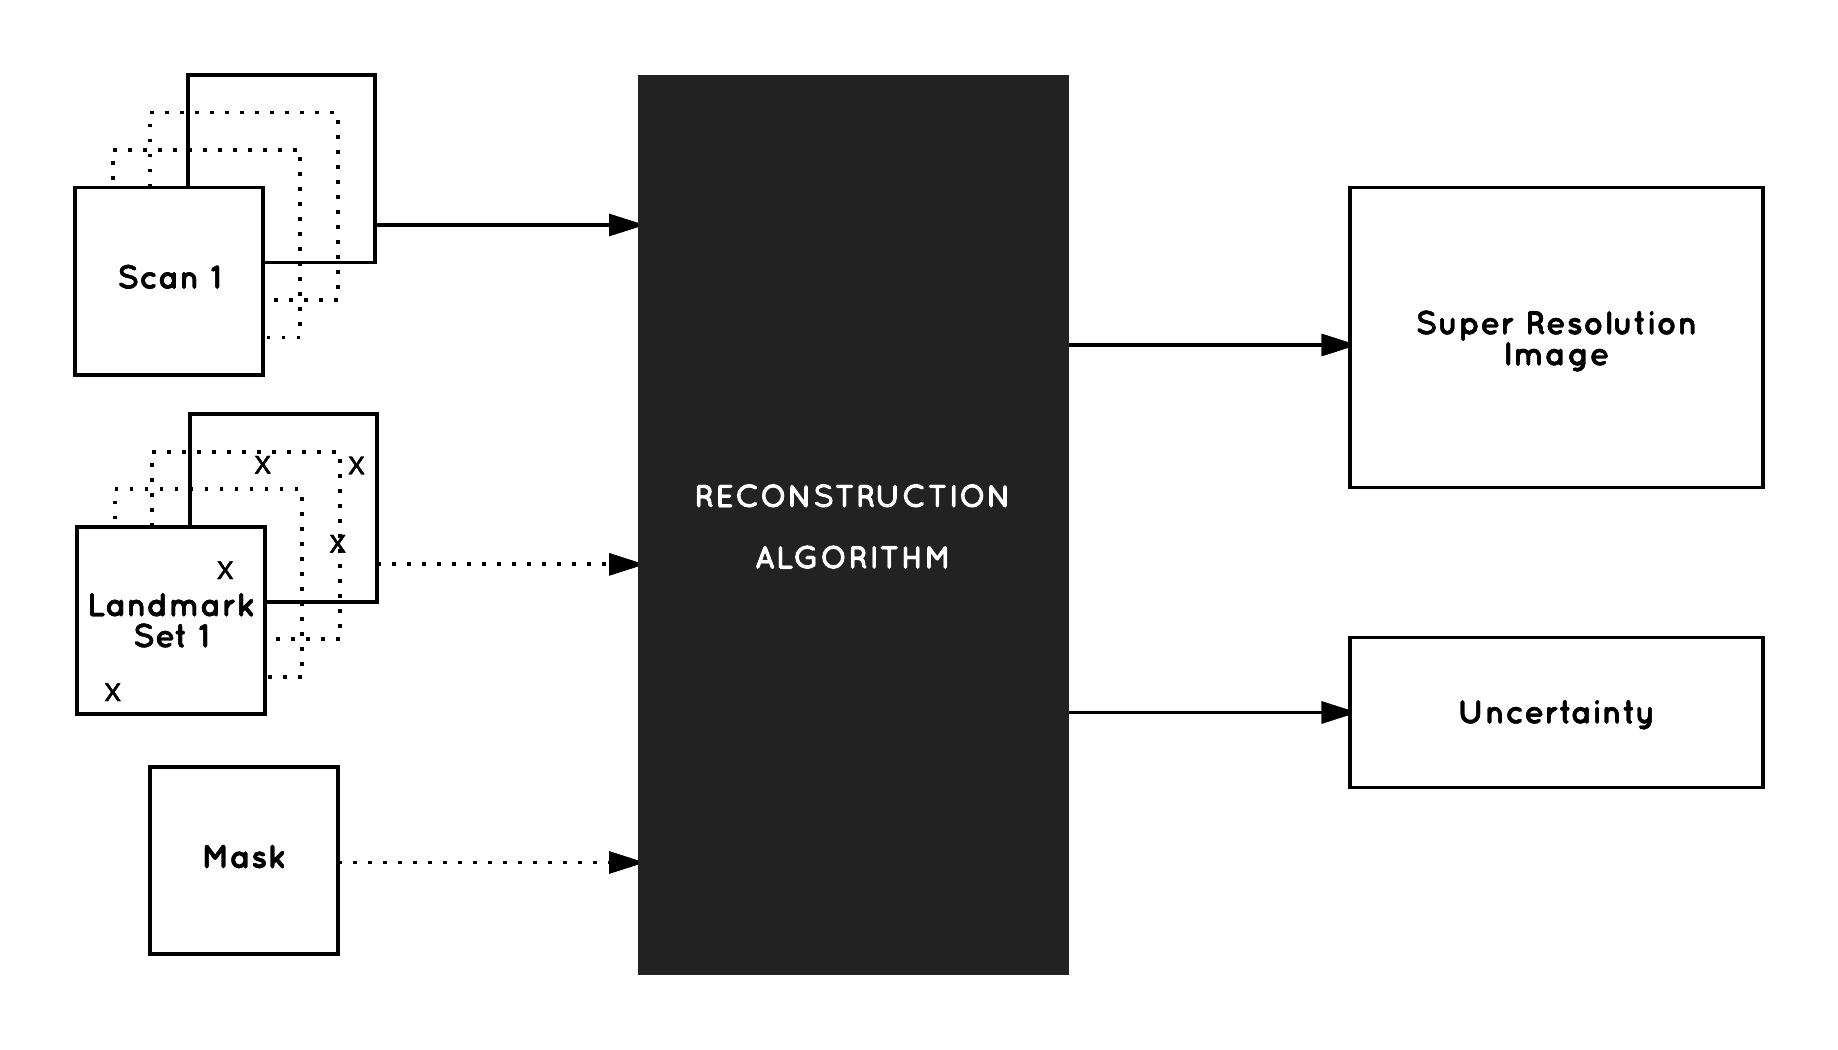
\includegraphics[width=0.8\textwidth]{images/reconstruction_overview.png}
  \caption{Reconstruction Overview}
  \label{fig:erosionbefore}
\end{figure}

The super resolution reconstruction process takes in a set of slice stacks (scans), an optional mask and outputs the reconstructed MRI volume and the uncertainty. The mask is used to ignore areas that are not of interest; for example when doing a fetal scan a mask can be created to ignore surrounding areas like the womb and amniotic fluid.

\section{Preprocessing}\label{section:preprocessing}
The uncertainty tells us for each pixel in the reconstructed volume how much confidence we have in that value. However, before we can visualize it some preprocessing must be applied. 

\subsection{Normalization}
The uncertainty is linearly scaled so each value is between 0 and 1.

\begin{verbatim}
  0 - no information (high uncertainty - worst)
  1 - maximum information (low uncertainty - best)
\end{verbatim}

\subsection{Erosion}
The optional erosion step removes the uncertainty values at the edge of the reconstruction. The edges often have a much higher uncertainty either because there are fewer slices to use or the mask cuts off the data required. Removing this edge helps the visualization to focus on the core of the volume.

The edges are removed in five steps:

\begin{enumerate}
  \item An erosion filter is applied to the image. This removes the edges but has the unwanted effect of also eroding uncertainty in the center of the volume.
  \item The absolute difference is taken between the original and the eroded image.
  \item The difference is then thresholded to create a mask of the areas that changed the most. The idea here is that the edges change significantly more than the small pockets of uncertainty inside.
  \item A growing filter is applied to the mask, to ensure the entire edge is covered.
  \item Finally all the points in the mask are set to 0 to remove the edge.
\end{enumerate}

Figure \ref{fig:erosionoverview} shows how the soft fade out of uncertainty due to the mask is removed to create a hard edge.

\begin{figure}[h]
  \centering
  \begin{subfigure}[b]{0.3\textwidth}
    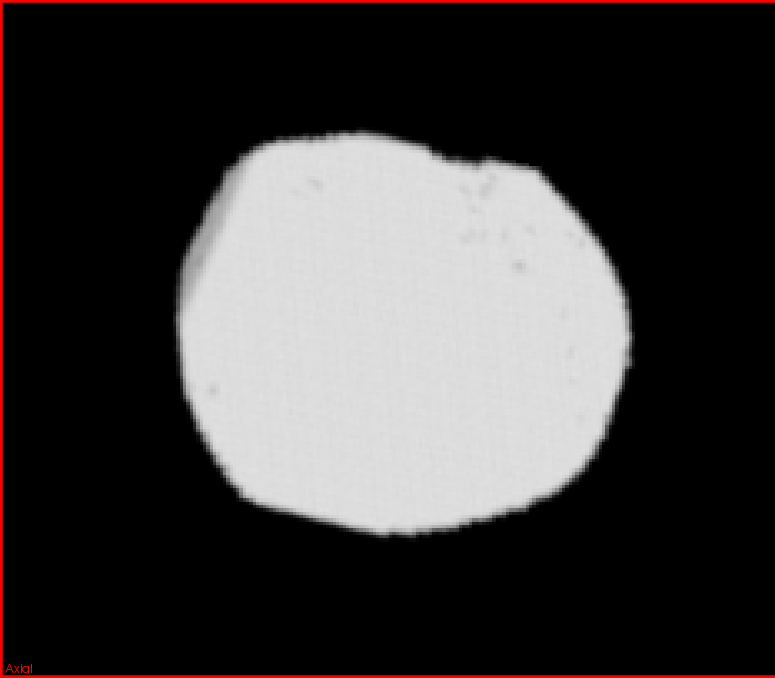
\includegraphics[width=\textwidth]{images/erosion/erosion_0.png}
    \caption{Original}
    \label{fig:erosion0}
  \end{subfigure}%
  ~ %add desired spacing between images, e. g. ~, \quad, \qquad, \hfill etc.
    %(or a blank line to force the subfigure onto a new line)
  \begin{subfigure}[b]{0.3\textwidth}
    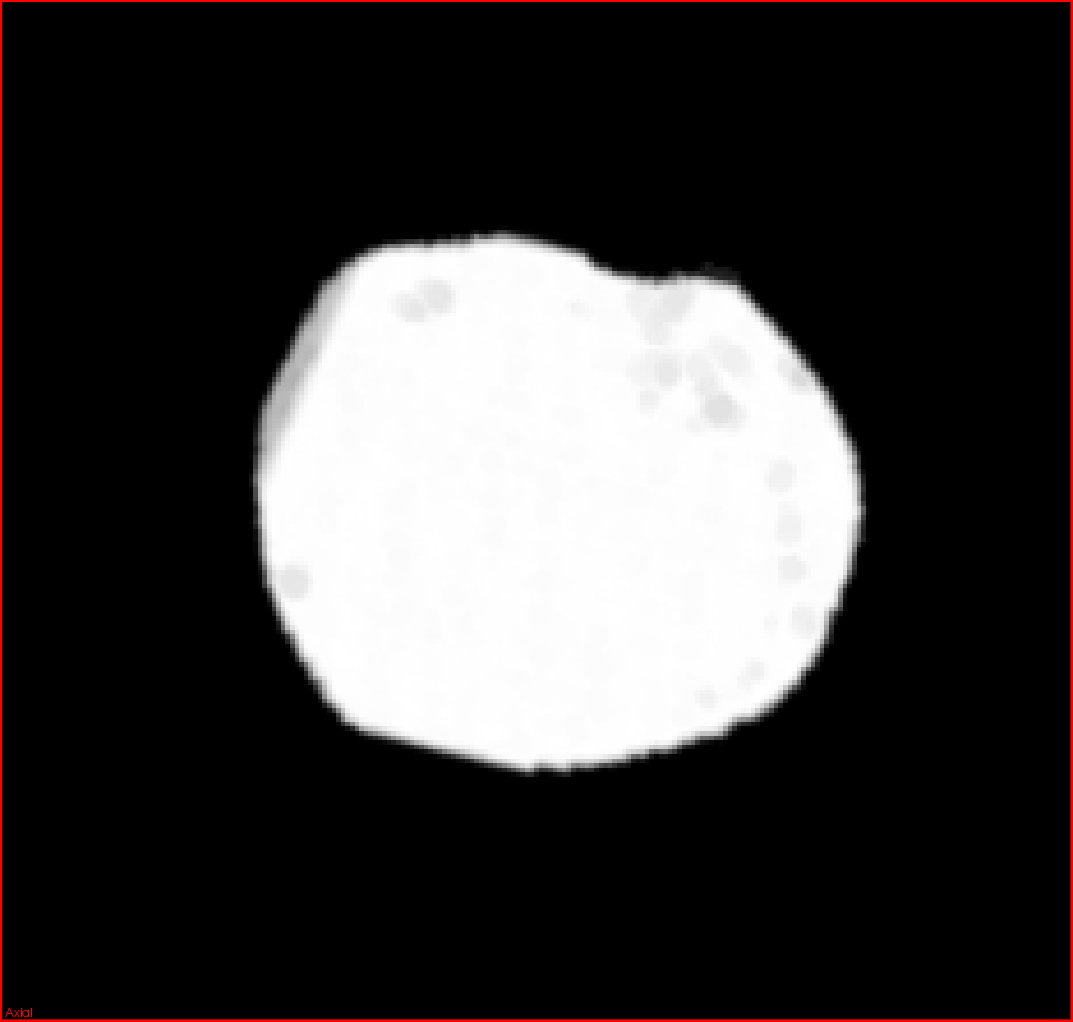
\includegraphics[width=\textwidth]{images/erosion/erosion_1.png}
    \caption{Step 1}
    \label{fig:erosion1}
  \end{subfigure}  
  ~ %add desired spacing between images, e. g. ~, \quad, \qquad, \hfill etc.
    %(or a blank line to force the subfigure onto a new line)
  \begin{subfigure}[b]{0.3\textwidth}
    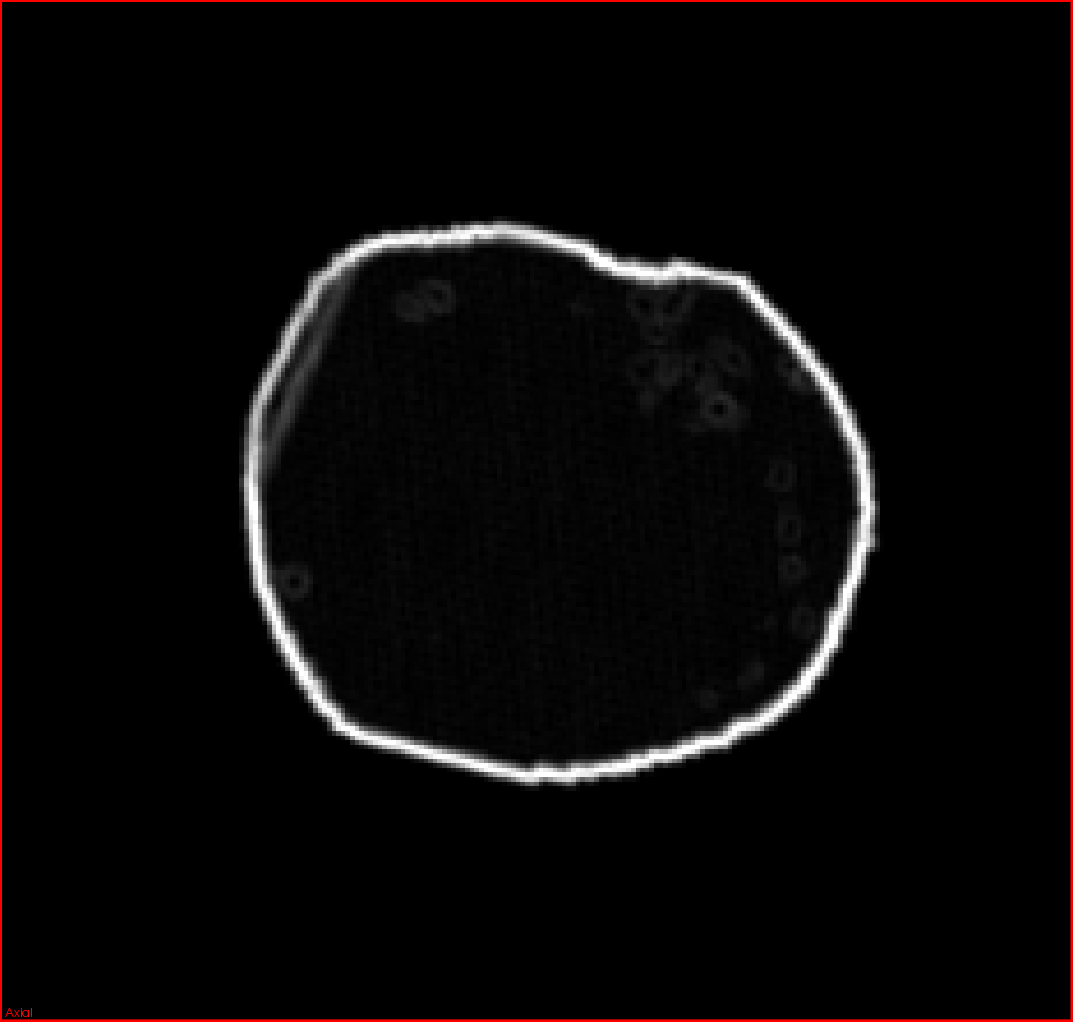
\includegraphics[width=\textwidth]{images/erosion/erosion_2.png}
    \caption{Step 2}
    \label{fig:erosion2}
  \end{subfigure}
  ~ %add desired spacing between images, e. g. ~, \quad, \qquad, \hfill etc.
    %(or a blank line to force the subfigure onto a new line)
  \begin{subfigure}[b]{0.3\textwidth}
    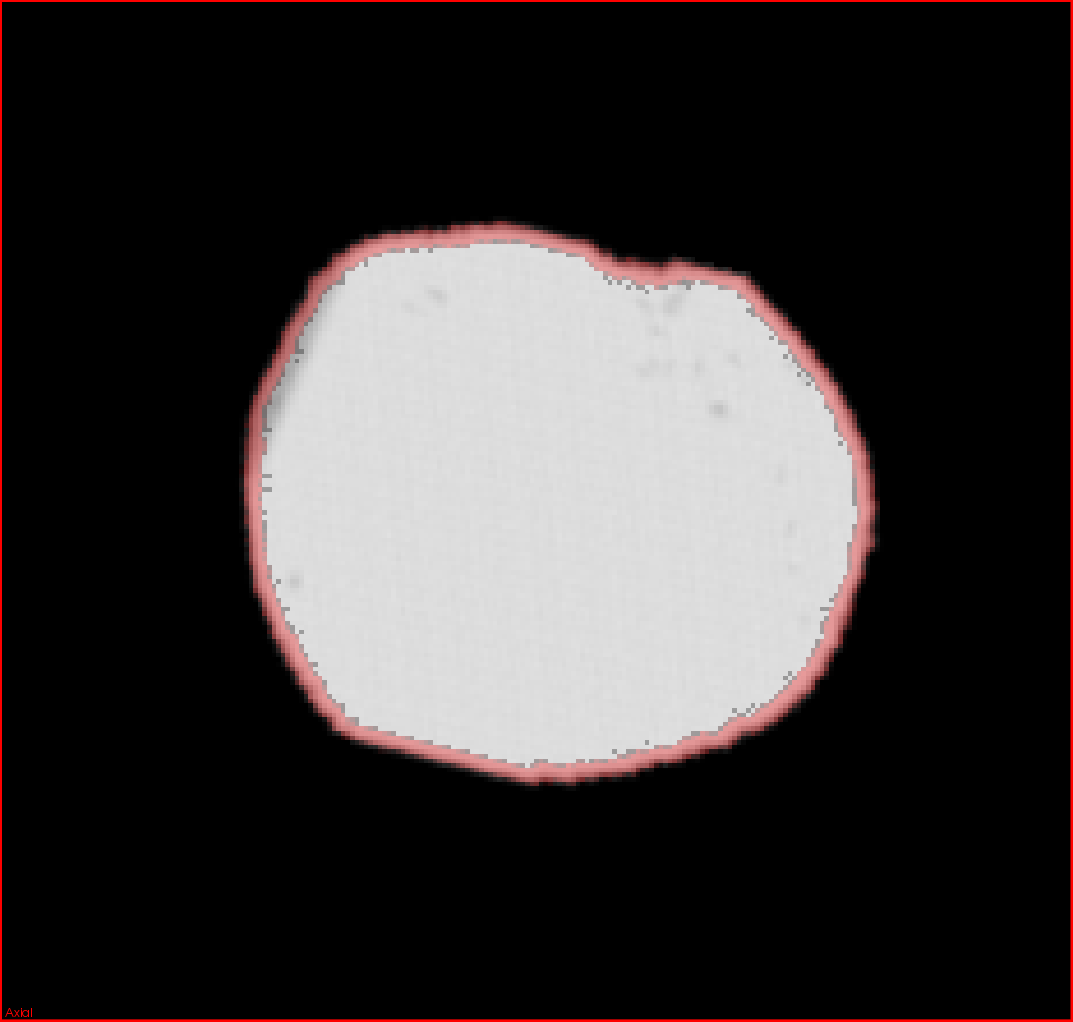
\includegraphics[width=\textwidth]{images/erosion/erosion_3.png}
    \caption{Step 3}
    \label{fig:erosion3}
  \end{subfigure}%
  ~ %add desired spacing between images, e. g. ~, \quad, \qquad, \hfill etc.
    %(or a blank line to force the subfigure onto a new line)
  \begin{subfigure}[b]{0.3\textwidth}
    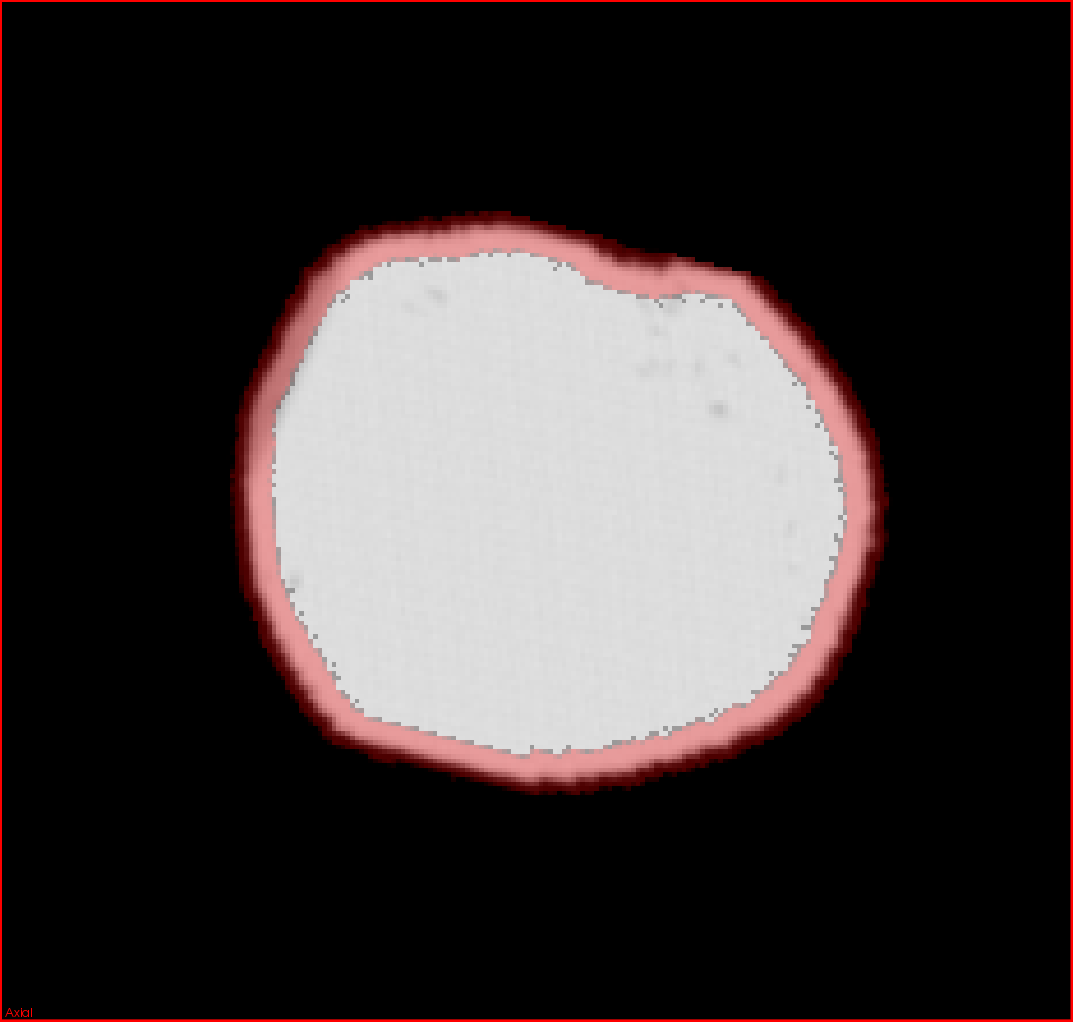
\includegraphics[width=\textwidth]{images/erosion/erosion_4.png}
    \caption{Step 4}
    \label{fig:erosion4}
  \end{subfigure}  
  ~ %add desired spacing between images, e. g. ~, \quad, \qquad, \hfill etc.
    %(or a blank line to force the subfigure onto a new line)
  \begin{subfigure}[b]{0.3\textwidth}
    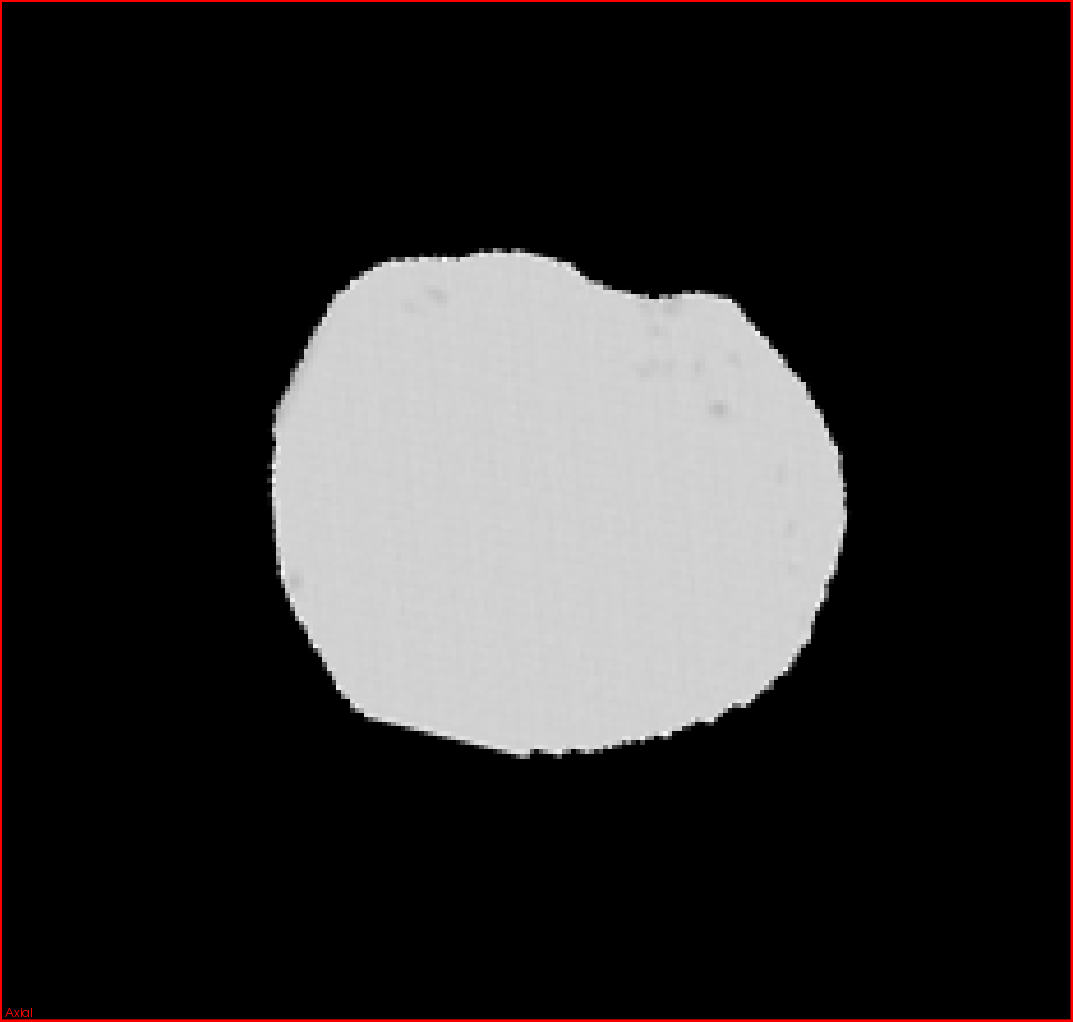
\includegraphics[width=\textwidth]{images/erosion/erosion_5.png}
    \caption{Step 5}
    \label{fig:erosion5}
  \end{subfigure}  
  \caption{Steps involved in removing the edge.}\label{fig:erosionoverview}
\end{figure}

\newpage
\section{Test Uncertainties}\label{section:testuncertainties}

To test the different visualizations during development a number of artificial uncertainty volumes were used, as well as an example fetal brain scan.

For each visualization that has been developed the results with these test uncertainties will be examined and compared.

\subsection{Sphere of Uncertainty}
An uncertainty volume where the uncertainty is proportional to the distance from the center. The uncertainty at the center is 0 (very uncertain) which then goes to 1 (very certain) at the edges.

\subsection{Sphere in Corner}
Similar to the sphere, but instead of being placed in the middle it is placed in one corner of the volume.

\subsection{Cube of Uncertainty}
An uncertainty volume that is 1 (very good) everywhere except for fixed size cube of uncertainty 0 (very bad) in the center.

\subsection{Random Uncertainty}
The uncertainty at every point is a random uniformly distributed value.

\subsection{Reconstruction Uncertainty}
Uncertainty generated from an example super resolution reconstruction of a fetal brain.\\

\begin{figure}[h]
  \centering
  \begin{subfigure}[b]{0.18\textwidth}
    \fcolorbox{gray}{white}{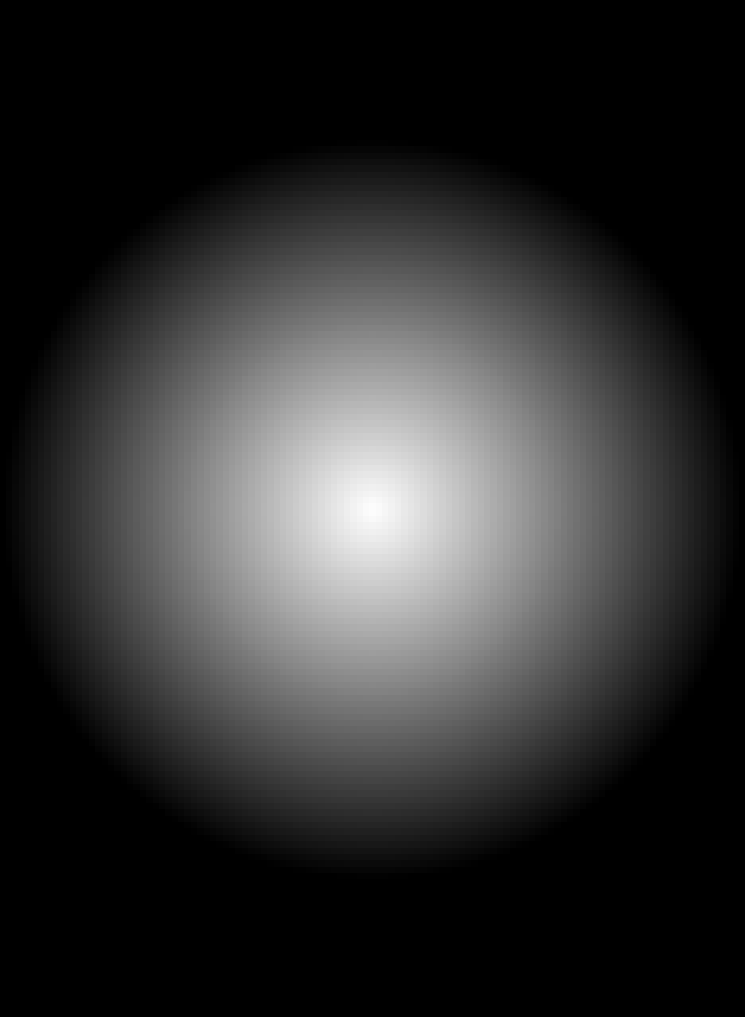
\includegraphics[width=\textwidth]{images/test/test_sphere.png}}
    \caption{Sphere}
    \label{fig:erosion0}
  \end{subfigure}%
  ~~%add desired spacing between images, e. g. ~, \quad, \qquad, \hfill etc.
    %(or a blank line to force the subfigure onto a new line)
  \begin{subfigure}[b]{0.18\textwidth}
    \fcolorbox{gray}{white}{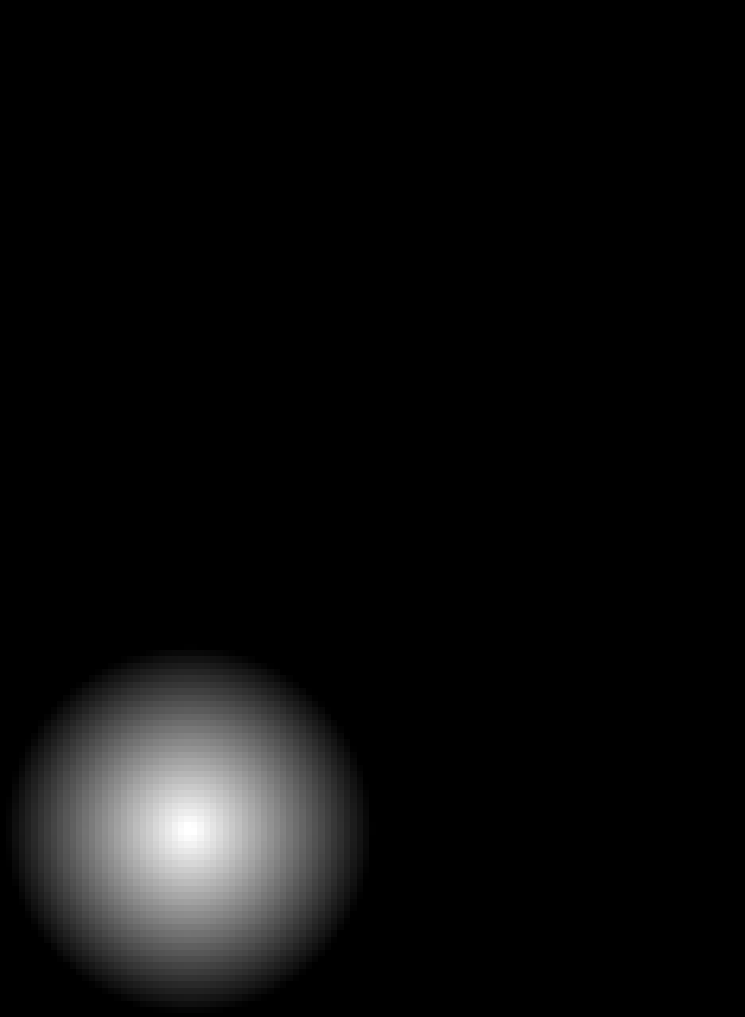
\includegraphics[width=\textwidth]{images/test/test_quadsphere.png}}
    \caption{Corner}
    \label{fig:erosion1}
  \end{subfigure}%
  ~~%add desired spacing between images, e. g. ~, \quad, \qquad, \hfill etc.
    %(or a blank line to force the subfigure onto a new line)
  \begin{subfigure}[b]{0.18\textwidth}
    \fcolorbox{gray}{white}{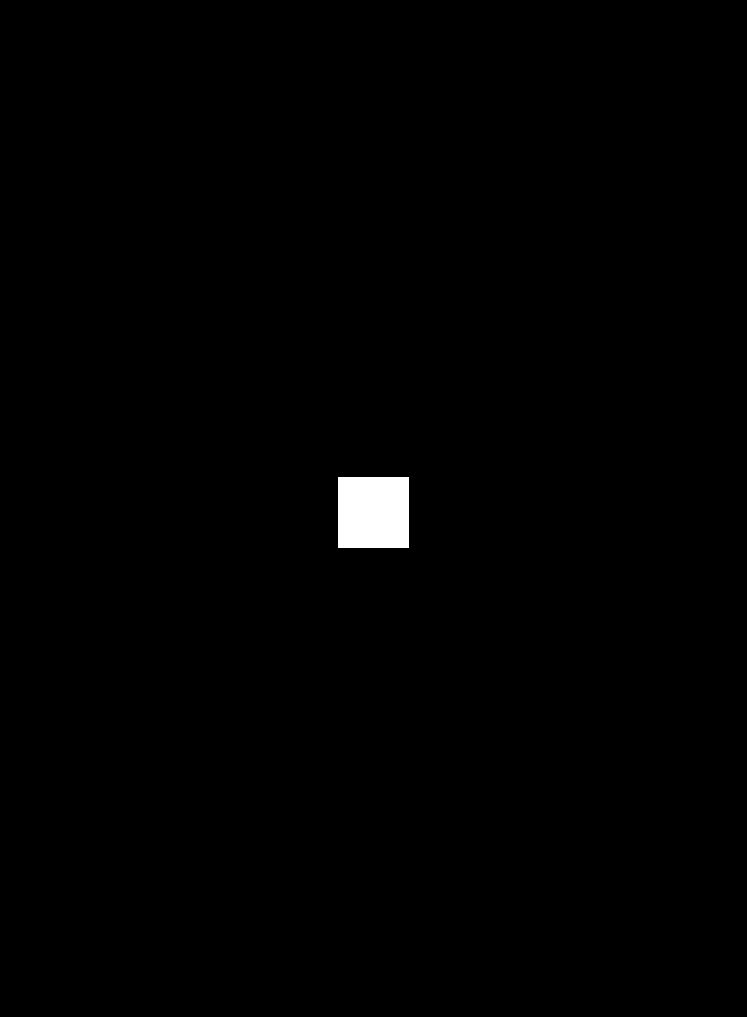
\includegraphics[width=\textwidth]{images/test/test_cube.png}}
    \caption{Cube}
    \label{fig:erosion2}
  \end{subfigure}%
  ~~%add desired spacing between images, e. g. ~, \quad, \qquad, \hfill etc.
    %(or a blank line to force the subfigure onto a new line)
  \begin{subfigure}[b]{0.18\textwidth}
    \fcolorbox{gray}{white}{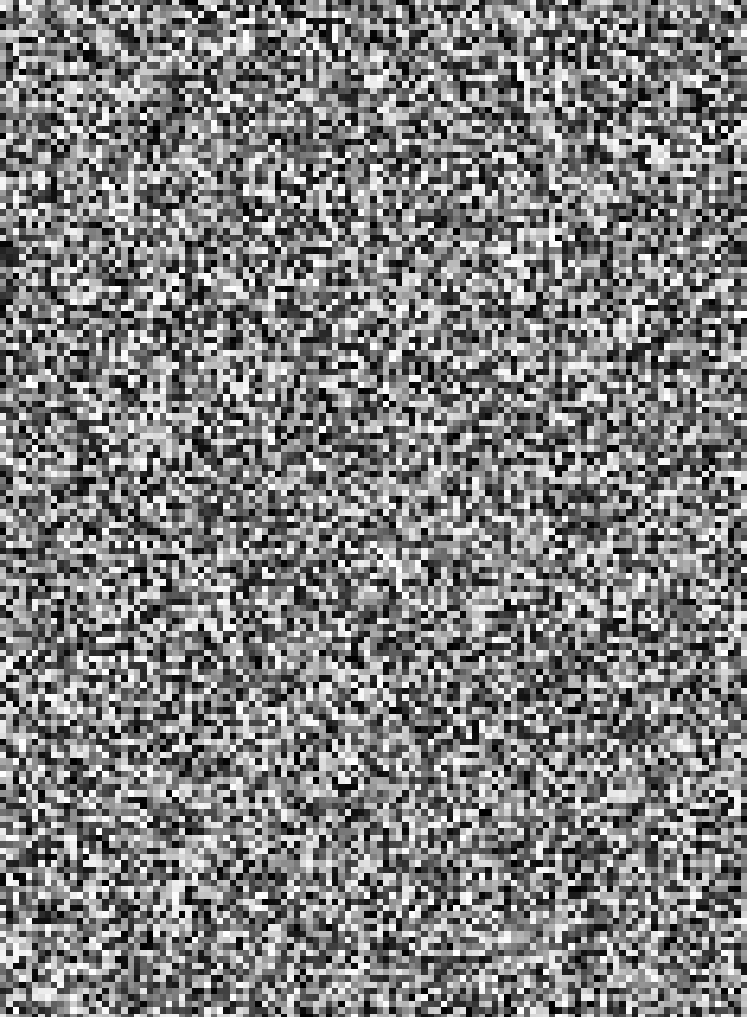
\includegraphics[width=\textwidth]{images/test/test_random.png}}
    \caption{Random}
    \label{fig:erosion3}
  \end{subfigure}%
  ~~%add desired spacing between images, e. g. ~, \quad, \qquad, \hfill etc.
    %(or a blank line to force the subfigure onto a new line)
  \begin{subfigure}[b]{0.18\textwidth}
    \fcolorbox{gray}{white}{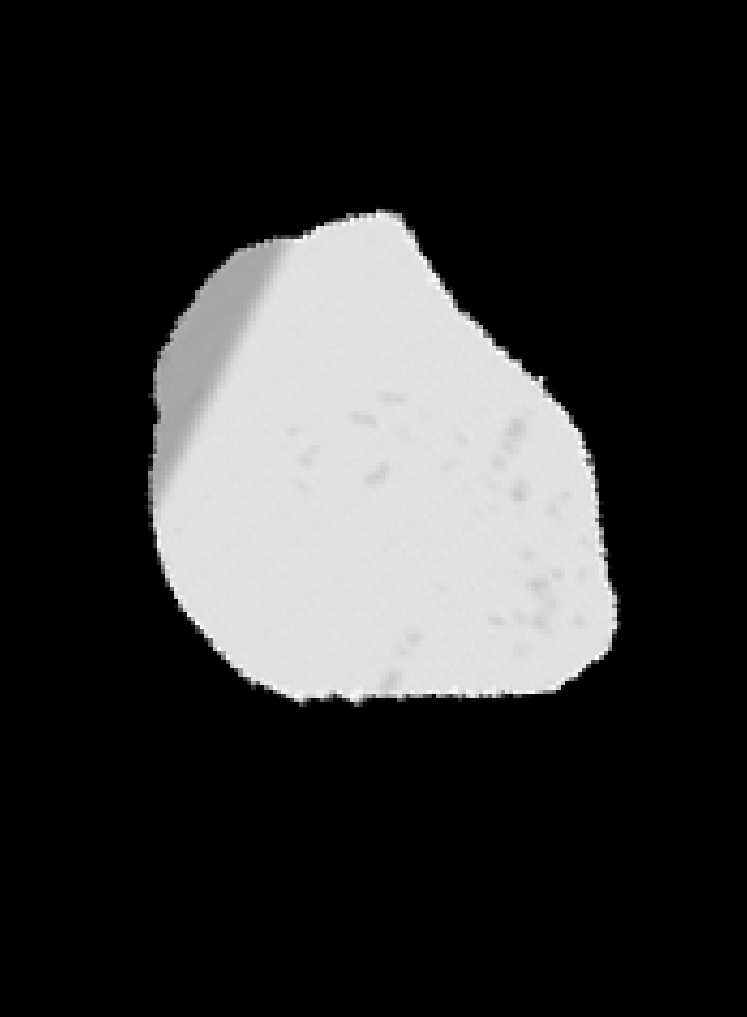
\includegraphics[width=\textwidth]{images/test/test_scan.png}}
    \caption{Scan}
    \label{fig:erosion3}
  \end{subfigure}
  \caption{Steps involved in removing the edge.}\label{fig:erosionoverview}
\end{figure}

% Idea -> Implementation -> Results
\newpage
\section{Thresholding}\label{section:thresholding}

The idea behind thresholding is to isolate areas in the reconstructed image within a particular range of uncertainty. This allows the viewer to highlight regions in a specified range (e.g. 0.2 to 0.5) and also lets them isolate the worst values in the volume (e.g. the worst 1$\%$).

\subsection*{Implementation}
The implementation uses a filter provided by ITK to go create a binary mask which is set to 1 where the uncertainty is in the range and 0 where it is not. This mask is then overlayed on the reconstructed scan in 2D and made transparent so both the uncertain area and underlying scan can be seen simultaneously. See figure \ref{fig:thresholding2d}.

\begin{figure}[H]
  \centering
  \begin{subfigure}[b]{0.3\textwidth}
    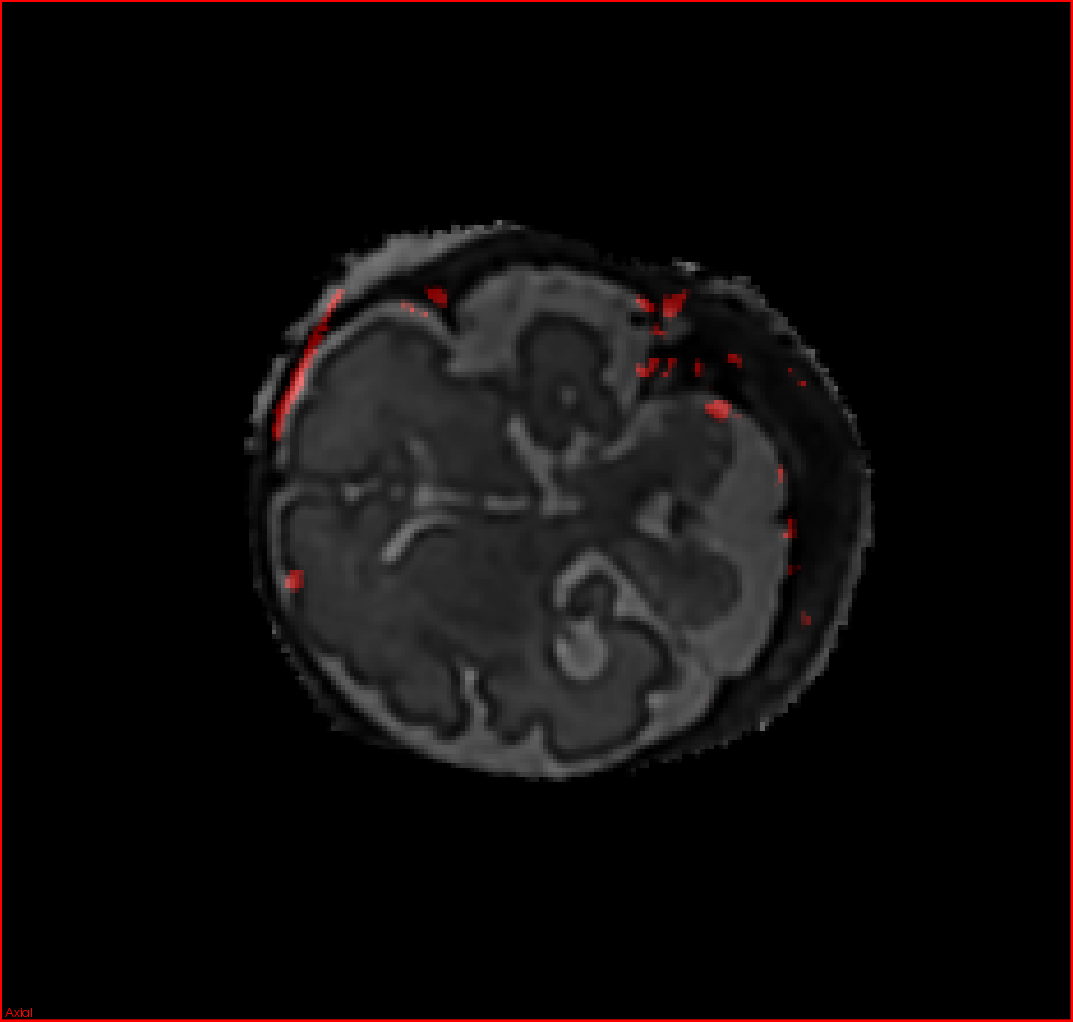
\includegraphics[width=\textwidth]{images/thresholding/thresholding_2d_axial.png}
    \caption{Axial}
    \label{fig:thresholding2daxial}
  \end{subfigure}%
  ~ %add desired spacing between images, e. g. ~, \quad, \qquad, \hfill etc.
    %(or a blank line to force the subfigure onto a new line)
  \begin{subfigure}[b]{0.3\textwidth}
    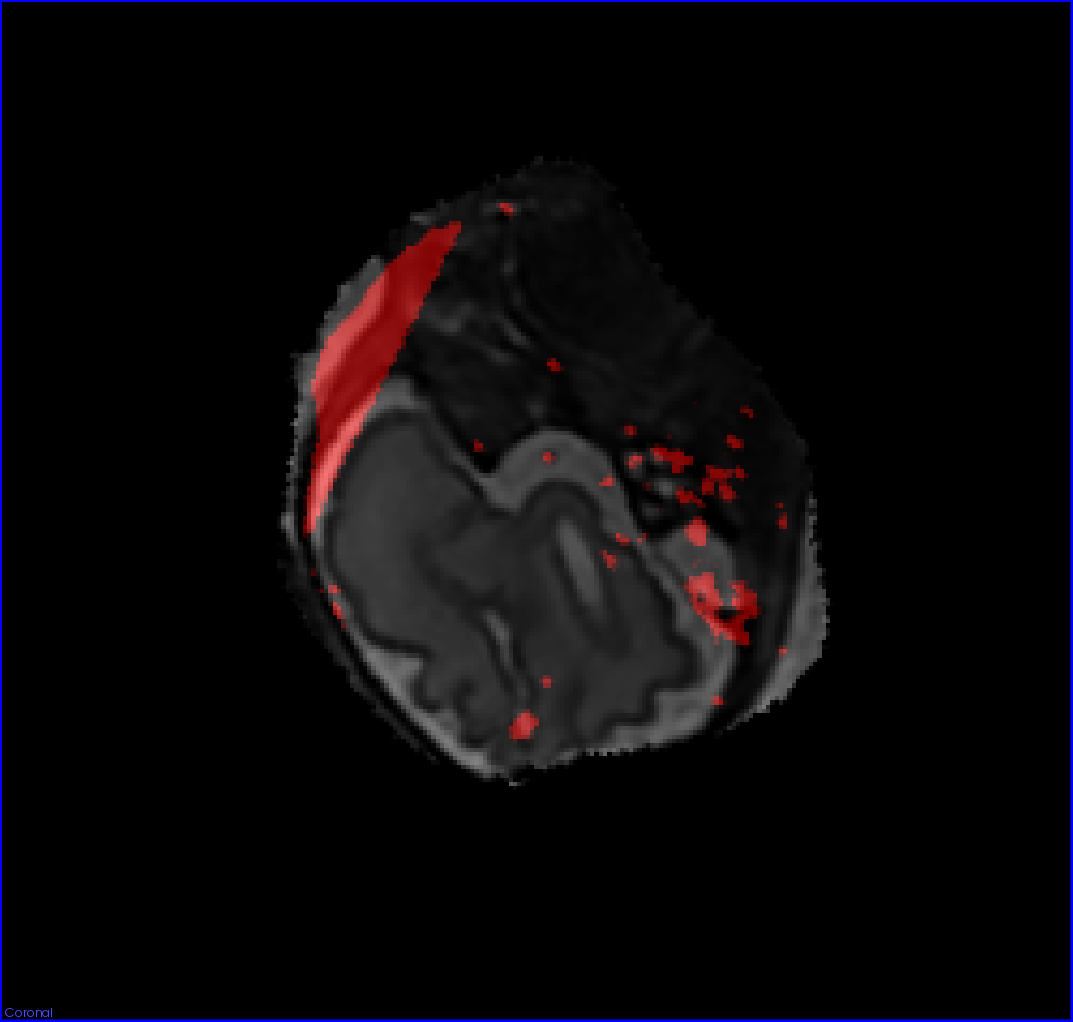
\includegraphics[width=\textwidth]{images/thresholding/thresholding_2d_coronal.png}
    \caption{Coronal}
    \label{fig:thresholding2dcoronal}
  \end{subfigure}%
  ~ %add desired spacing between images, e. g. ~, \quad, \qquad, \hfill etc.
    %(or a blank line to force the subfigure onto a new line)
  \begin{subfigure}[b]{0.3\textwidth}
    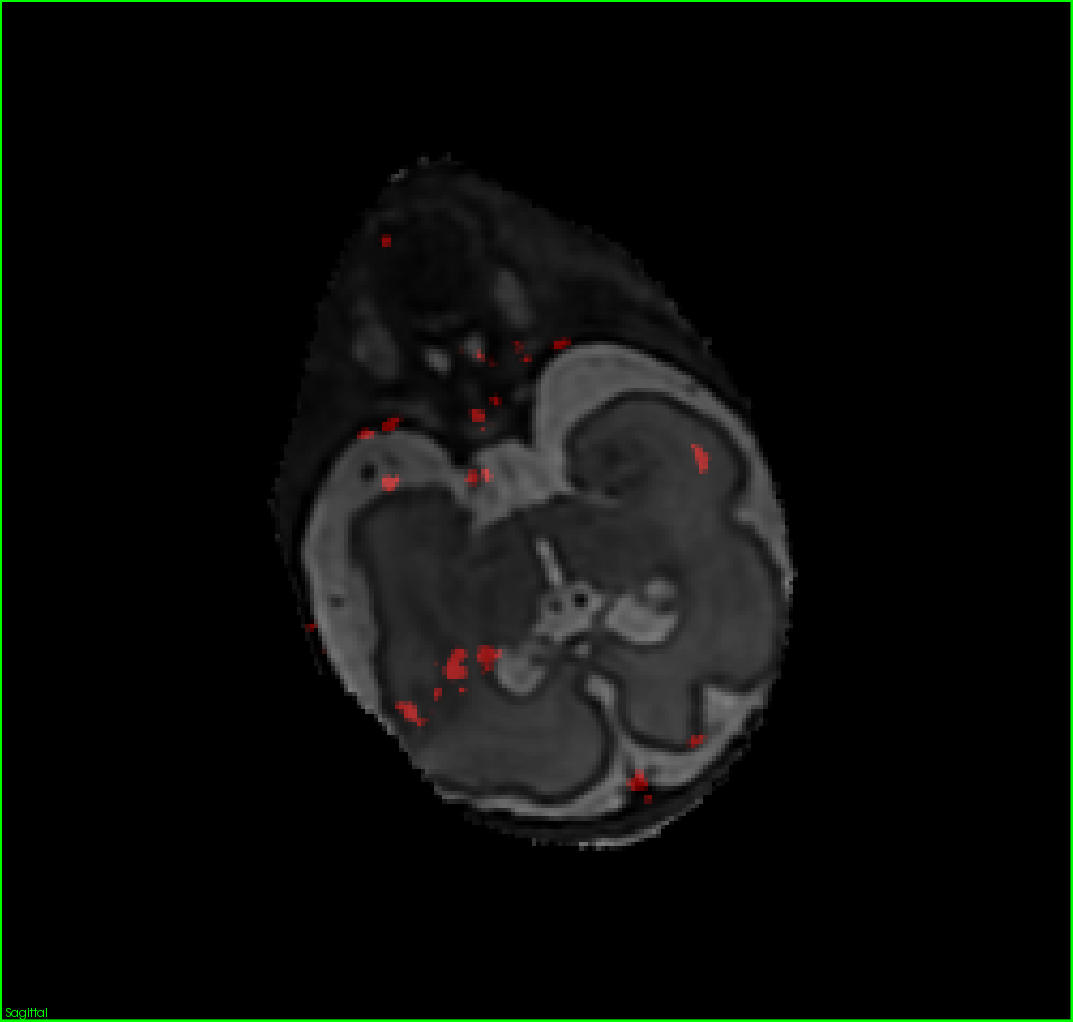
\includegraphics[width=\textwidth]{images/thresholding/thresholding_2d_sagittal.png}
    \caption{Sagittal}
    \label{fig:thresholding2dsagittal}  
  \end{subfigure}
  \caption{Thresholding in 2D}\label{fig:thresholding2d}
\end{figure}

To view the uncertainty in 3D, two variations have been implemented, both using volume rendering (see section \ref{background:volumerendering}). Variation 1 applies volume rendering directly to the uncertainty and variation 2 applies volume rendering to the binary mask.

The transfer functions used in each variation can be seen in figure \ref{fig:thresholdingoverview}. The first works by making values within the thresholded range opaque and those outside it transparent. The second works in a similar way; 0 in the mask is out of the range and 1 in the mask is in the range. In the second transfer function there is a slow fade out, rather than a sharp change, to give individual points of uncertainty some presence.

\begin{figure}[H]
  \centering
  \begin{subfigure}[b]{0.5\textwidth}
    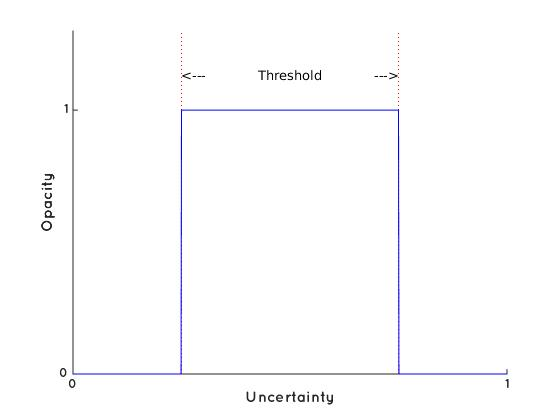
\includegraphics[width=\textwidth]{images/thresholding/thresholdvariation1.jpg}
    \caption{Variation 1}
    \label{fig:thresholdingvariation1}
  \end{subfigure}%
  ~ %add desired spacing between images, e. g. ~, \quad, \qquad, \hfill etc.
    %(or a blank line to force the subfigure onto a new line)
  \begin{subfigure}[b]{0.5\textwidth}
    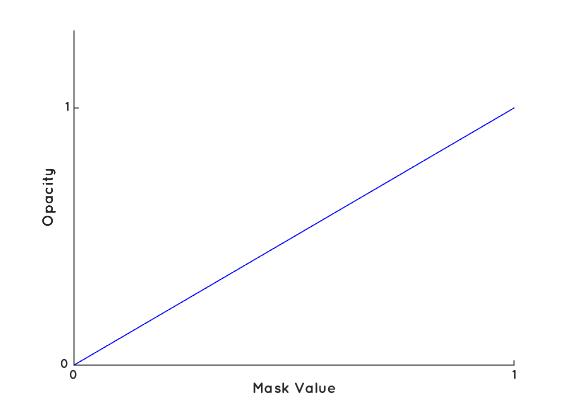
\includegraphics[width=\textwidth]{images/thresholding/thresholdvariation2.jpg}
    \caption{Variation 2}
    \label{fig:thresholdingvariation2}
  \end{subfigure}
  \caption{Opacity Transfer Functions. Opacity of 0 is transparent, 1 is opaque.}\label{fig:thresholdingoverview}
\end{figure}

An issue found with variation 1 was that the renderer still draws the edge of the uncertainty, even though it had previously been removed by erosion. This is due to the renderer using linear interpolation to take samples along each ray fired into the volume. Figure \ref{fig:thresholdingvariation1problem} illustrates the problem - the background has uncertainty 0.0, and the object has uncertainty $~$0.6. Points interpolated between the two will lie in the range 0.0-0.6 and so we find values of uncertainty that don't actually exist in the object.

\begin{figure}[h]
  \centering
  \begin{subfigure}[b]{0.5\textwidth}
    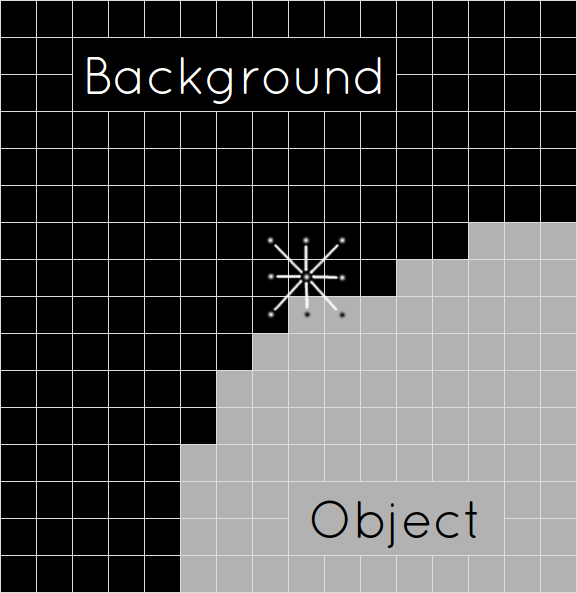
\includegraphics[width=\textwidth]{images/thresholding/thresholdvariation1example.png}
    \caption{Simplified View}
    \label{fig:thresholdingvariation1example}
  \end{subfigure}%
  ~ %add desired spacing between images, e. g. ~, \quad, \qquad, \hfill etc.
    %(or a blank line to force the subfigure onto a new line)
  \begin{subfigure}[b]{0.5\textwidth}
    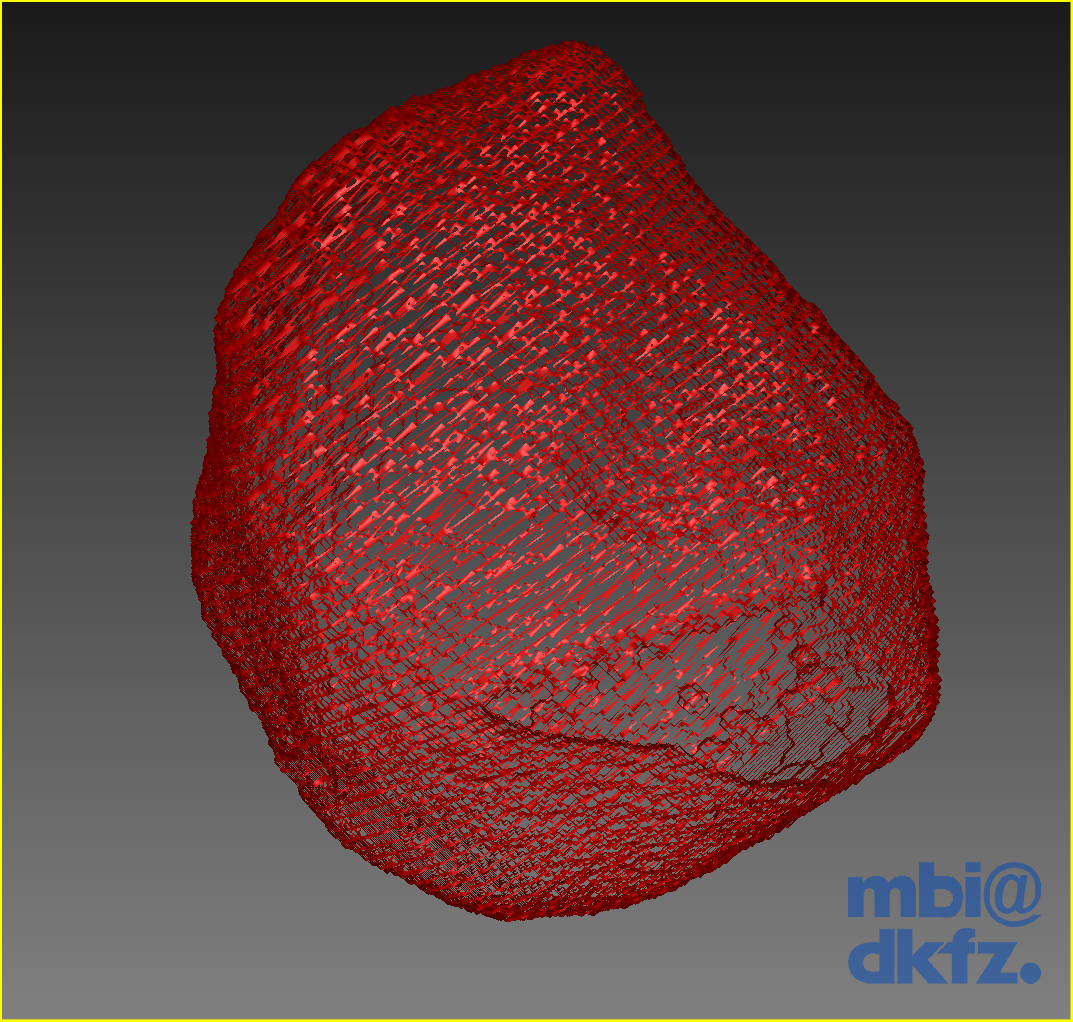
\includegraphics[width=\textwidth]{images/thresholding/thresholdvariation1problem.png}
    \caption{Edge Artefacts}
    \label{fig:thresholdingvariation1artefacts}
  \end{subfigure}
  \caption{Opacity Transfer Functions. Opacity of 0 is transparent, 1 is opaque.}\label{fig:thresholdingvariation1problem}
\end{figure}

A solution to this problem is to use a gradient transfer function which allows the change in uncertainty to influence the transparency. Rapid changes in uncertainty can therefore be treated as noise and ignored. The cutoff can be adjusted to remove the entire edge but there is a tradeoff as some genuine regions of uncertainty can also be filteredout. Figure \ref{fig:thresholdingvariationfix} shows the transfer function and the effect of tweaking the threshold.

\begin{figure}[H]
  \centering
  \begin{subfigure}[b]{0.5\textwidth}
    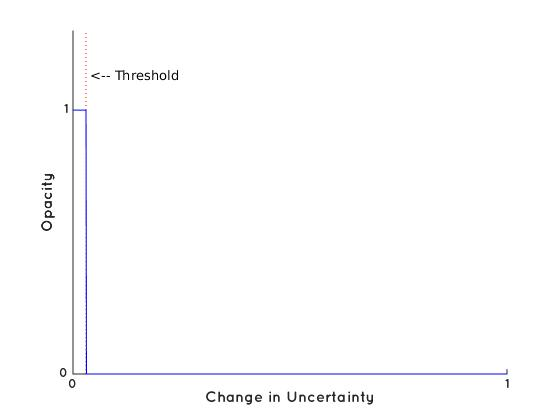
\includegraphics[width=\textwidth]{images/thresholding/thresholdvariation1fix.jpg}
    \caption{Gradient Transfer Function}
    \label{fig:thresholdingvariation1example}
  \end{subfigure}%
  ~ %add desired spacing between images, e. g. ~, \quad, \qquad, \hfill etc.
    %(or a blank line to force the subfigure onto a new line)
  \begin{subfigure}[b]{0.5\textwidth}
    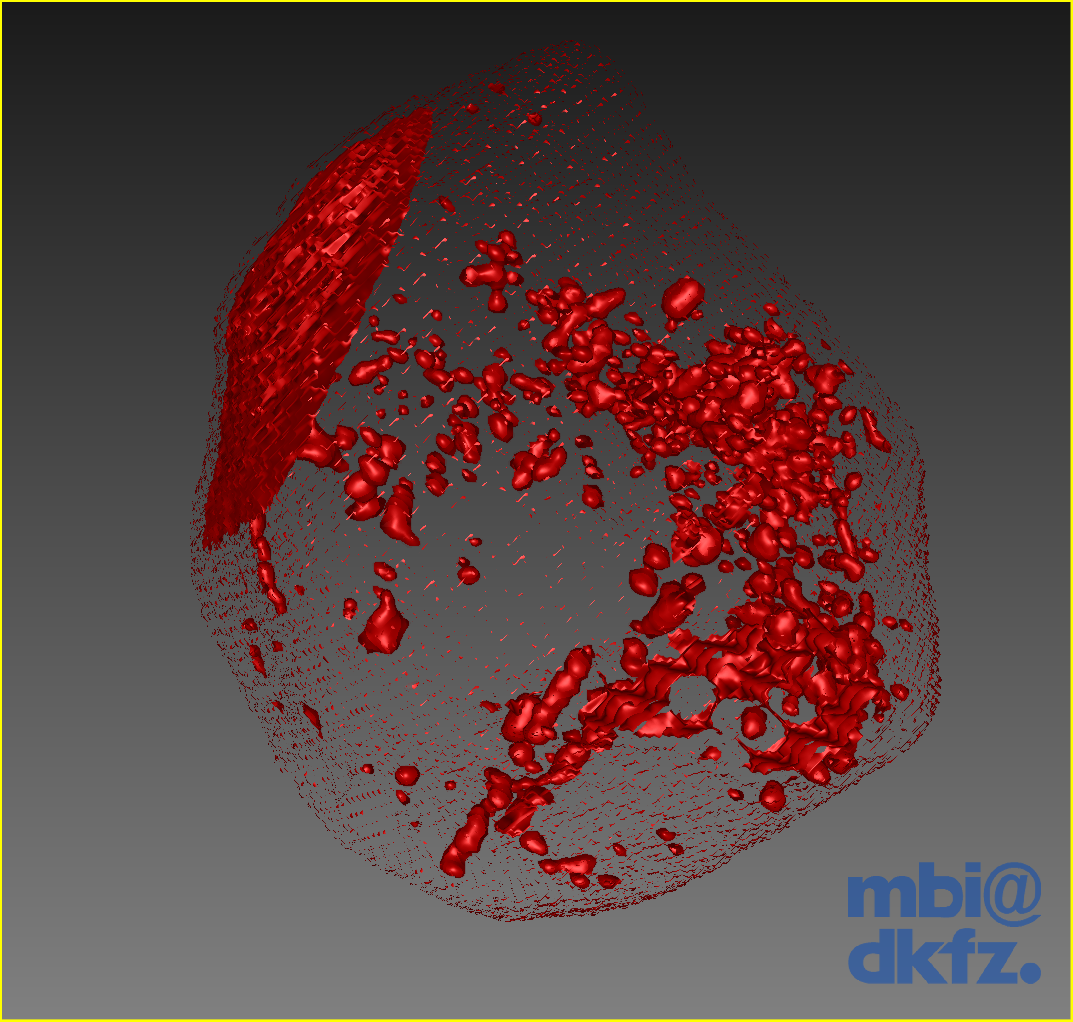
\includegraphics[width=\textwidth]{images/thresholding/thresholdvariation1threshold1.png}
    \caption{Threshold 0.05}
    \label{fig:thresholdingvariation1threshold1}
  \end{subfigure}
  ~%add desired spacing between images, e. g. ~, \quad, \qquad, \hfill etc.
    %(or a blank line to force the subfigure onto a new line)
  \begin{subfigure}[b]{0.5\textwidth}
    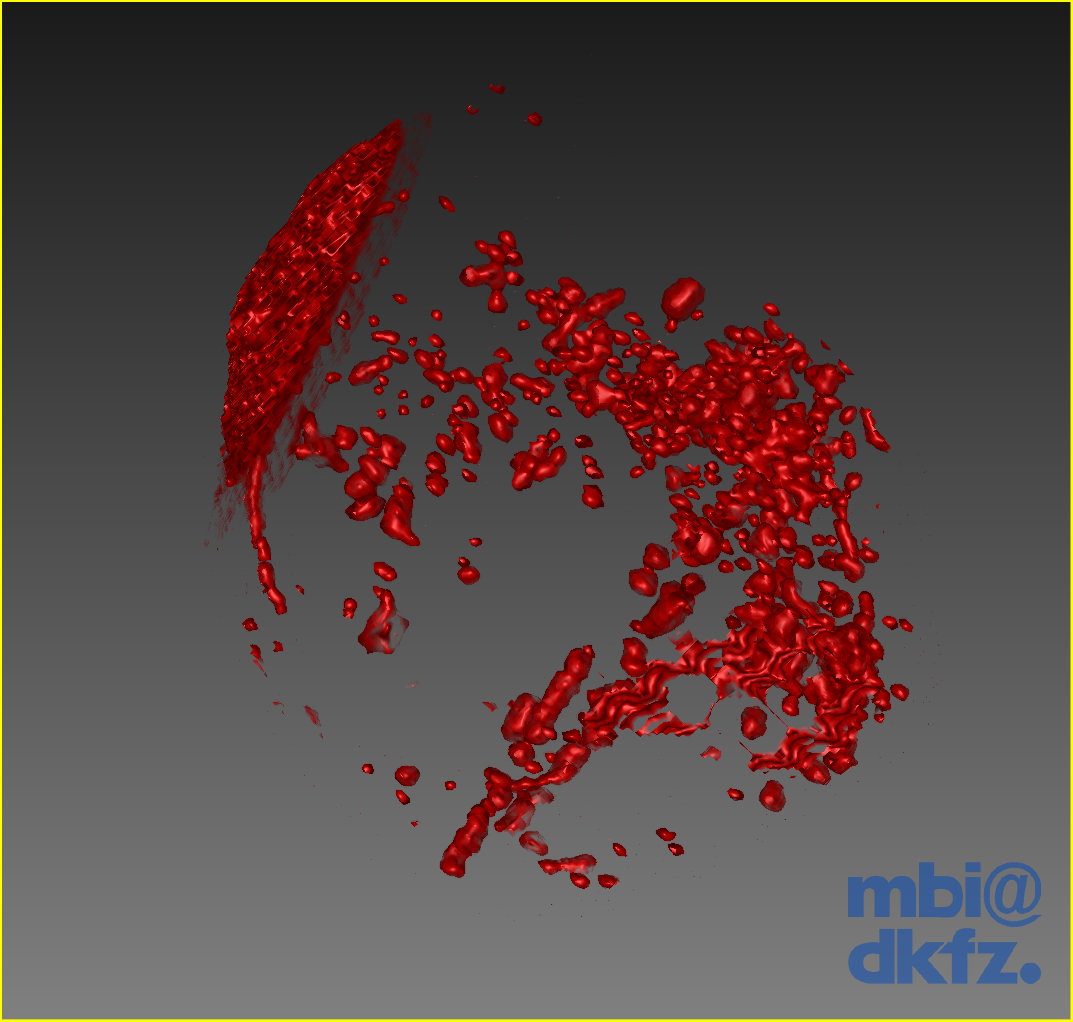
\includegraphics[width=\textwidth]{images/thresholding/thresholdvariation1threshold2.png}
    \caption{Threshold 0.02}
    \label{fig:thresholdingvariation1threshold2}  
  \end{subfigure}%
  ~ %add desired spacing between images, e. g. ~, \quad, \qquad, \hfill etc.
    %(or a blank line to force the subfigure onto a new line)
  \begin{subfigure}[b]{0.5\textwidth}
    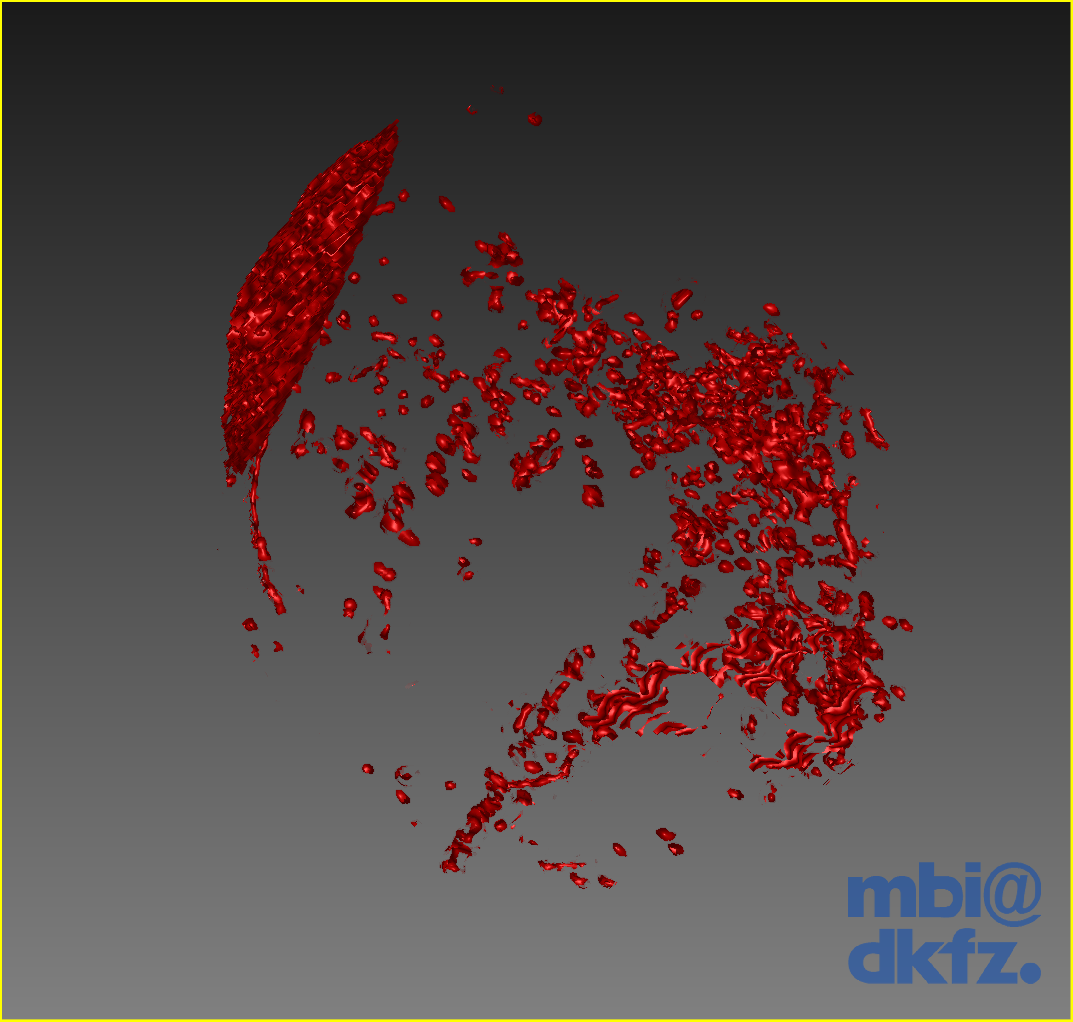
\includegraphics[width=\textwidth]{images/thresholding/thresholdvariation1threshold3.png}
    \caption{Threshold 0.01}
    \label{fig:thresholdingvariation1threshold3}  
  \end{subfigure}  
  \caption{Reducing the threshold removes the edge but removes some uncertainty.}\label{fig:thresholdingvariationfix}
\end{figure}

Although tweaking the threshold can remove edge artefact variation 2 was found not to exhibit these problems and so this implementation was used in the evaluation of the prototype.

\newpage
\subsection*{Results}
Here are the results that are achieved with the test uncertainties (see section \ref{section:testuncertainties}).

\begin{figure}[H]
  \centering
  \begin{subfigure}[b]{0.32\textwidth}
    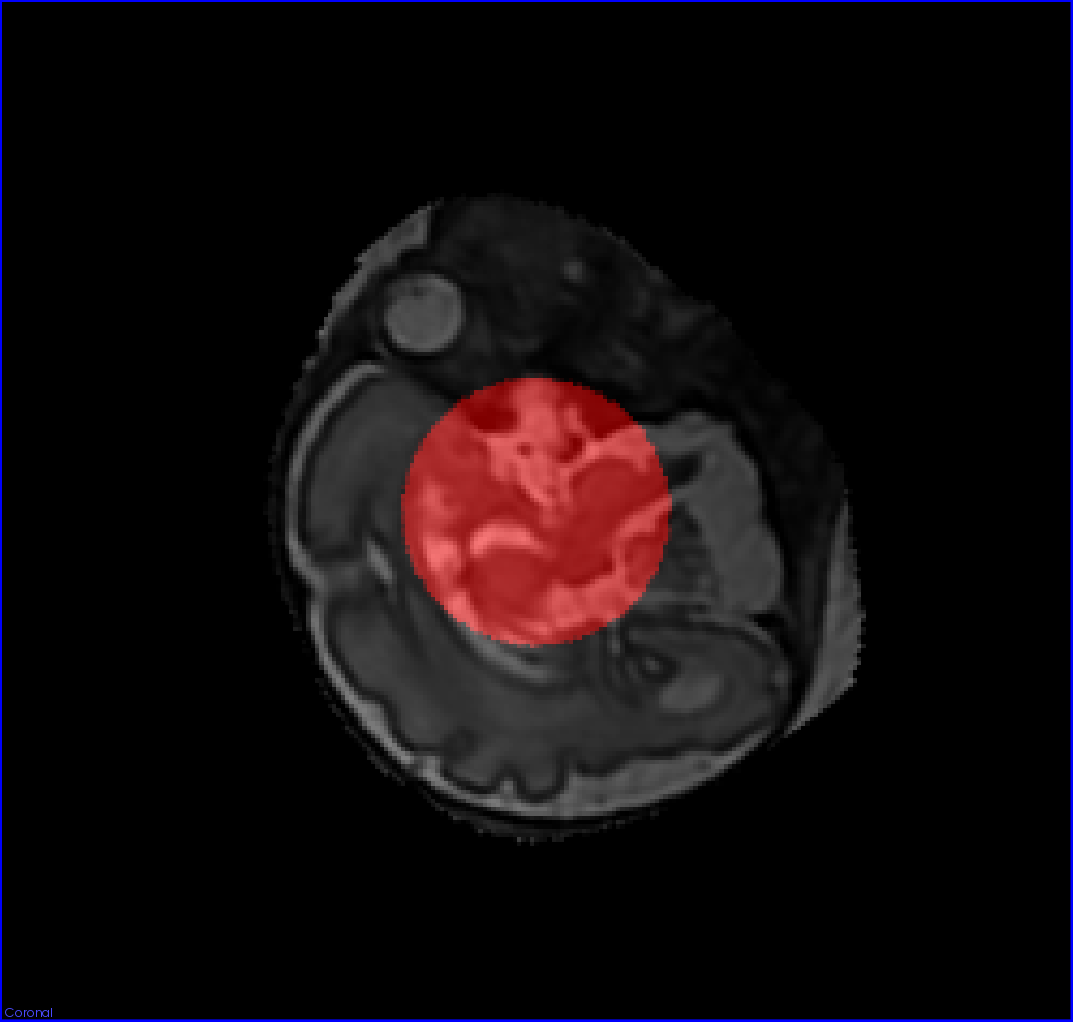
\includegraphics[width=\textwidth]{images/thresholding/results/sphere_2d.png}
    \caption{Sphere in 2D}
    \label{fig:thresholdingresultssphere2d}
  \end{subfigure}%
  ~ %add desired spacing between images, e. g. ~, \quad, \qquad, \hfill etc.
    %(or a blank line to force the subfigure onto a new line)
  \begin{subfigure}[b]{0.32\textwidth}
    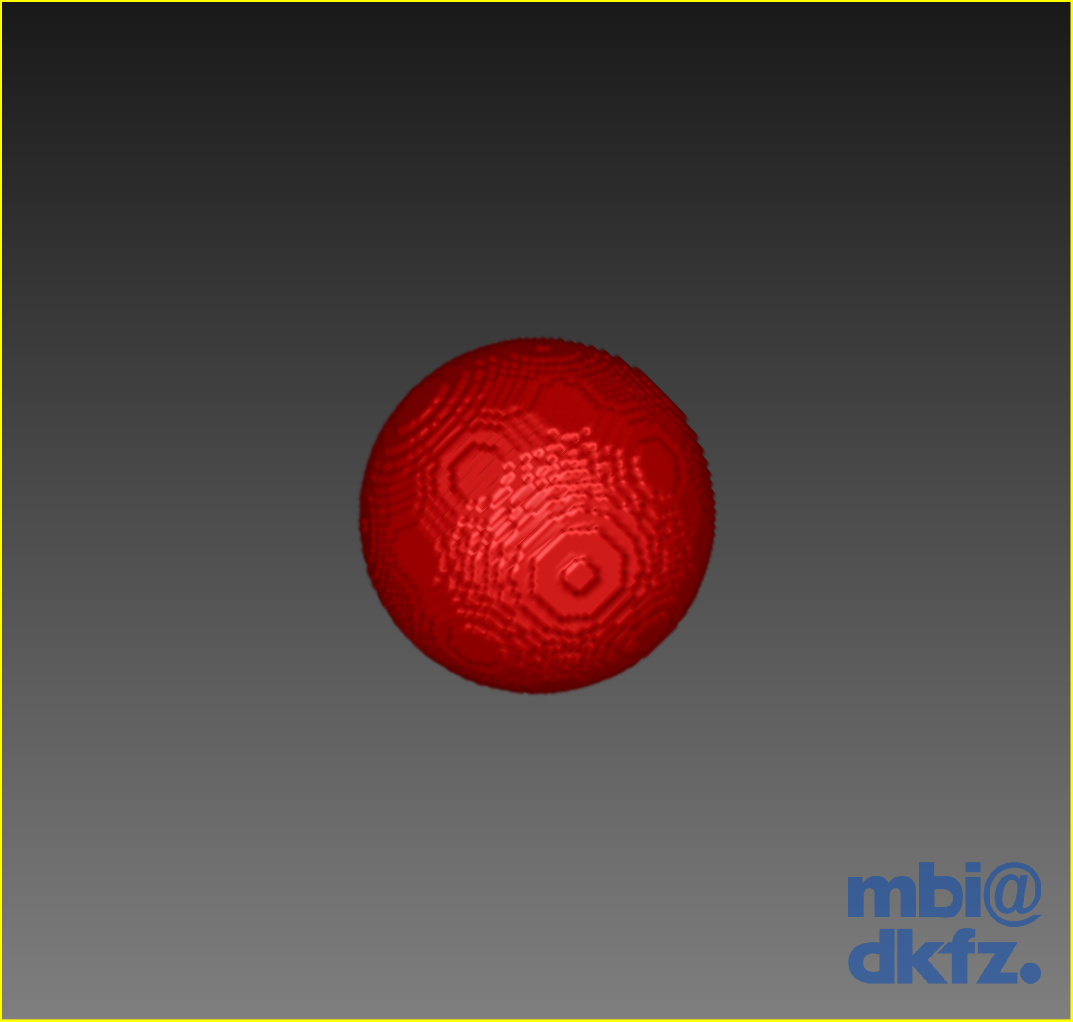
\includegraphics[width=\textwidth]{images/thresholding/results/sphere_3d.png}
    \caption{Sphere in 3D}
    \label{fig:thresholdingresultssphere3d}
  \end{subfigure}
  ~ %add desired spacing between images, e. g. ~, \quad, \qquad, \hfill etc.
    %(or a blank line to force the subfigure onto a new line)
  \begin{subfigure}[b]{0.32\textwidth}
    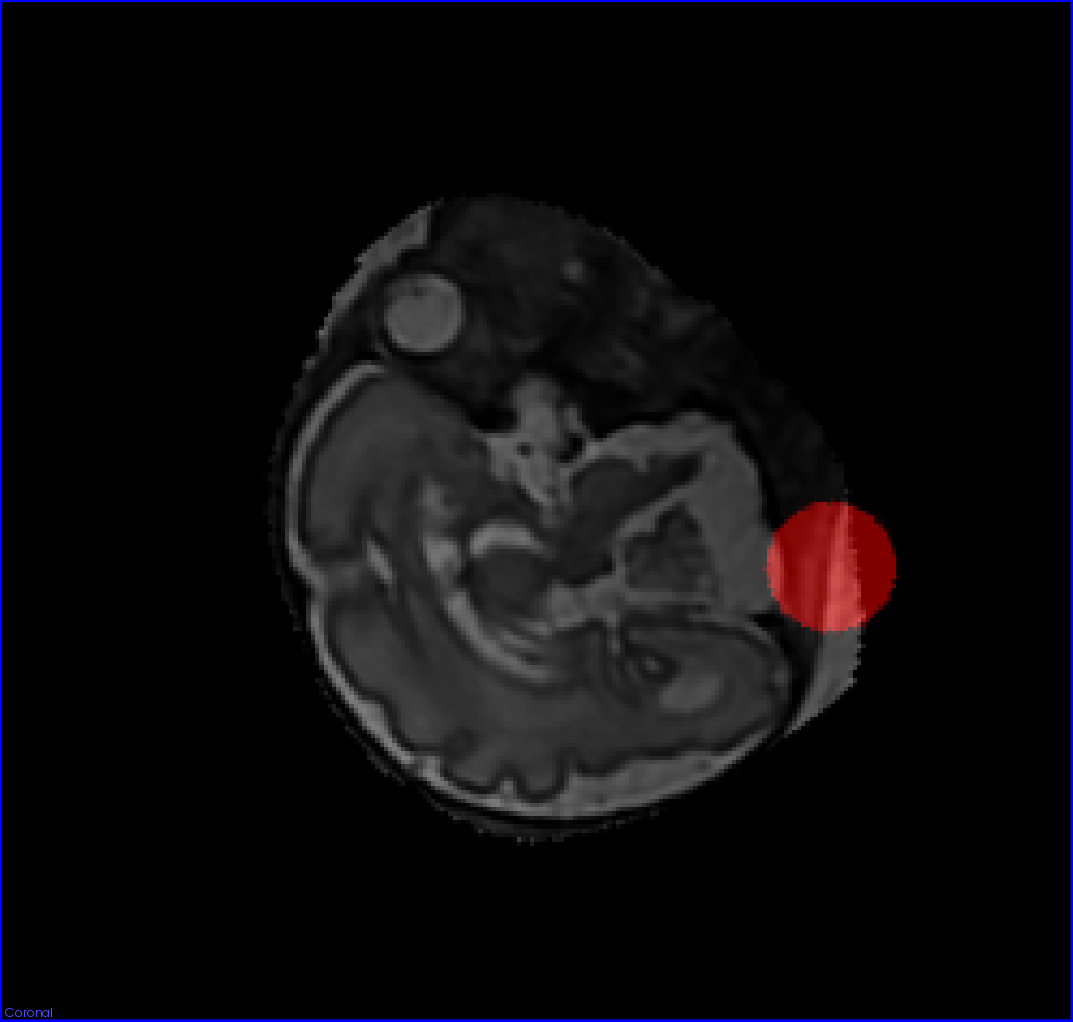
\includegraphics[width=\textwidth]{images/thresholding/results/sphere_corner_2d.png}
    \caption{Sphere in Corner in 2D}
    \label{fig:thresholdingresultsspherecorner2d}
  \end{subfigure}%
  ~ %add desired spacing between images, e. g. ~, \quad, \qquad, \hfill etc.
    %(or a blank line to force the subfigure onto a new line)
  \begin{subfigure}[b]{0.32\textwidth}
    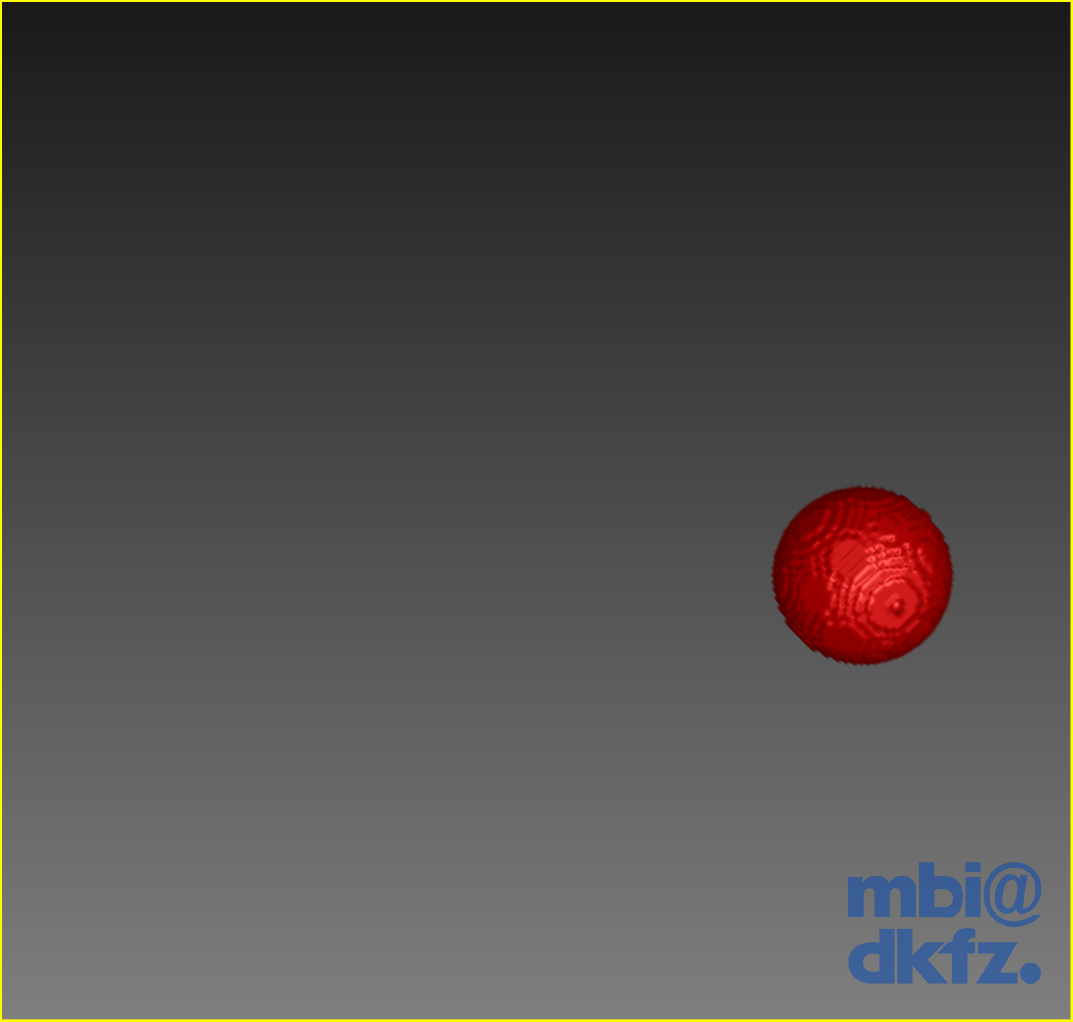
\includegraphics[width=\textwidth]{images/thresholding/results/sphere_corner_3d.png}
    \caption{Sphere in Corner in 3D}
    \label{fig:thresholdingresultsspherecorner3d}
  \end{subfigure}
  ~ %add desired spacing between images, e. g. ~, \quad, \qquad, \hfill etc.
    %(or a blank line to force the subfigure onto a new line)
  \begin{subfigure}[b]{0.32\textwidth}
    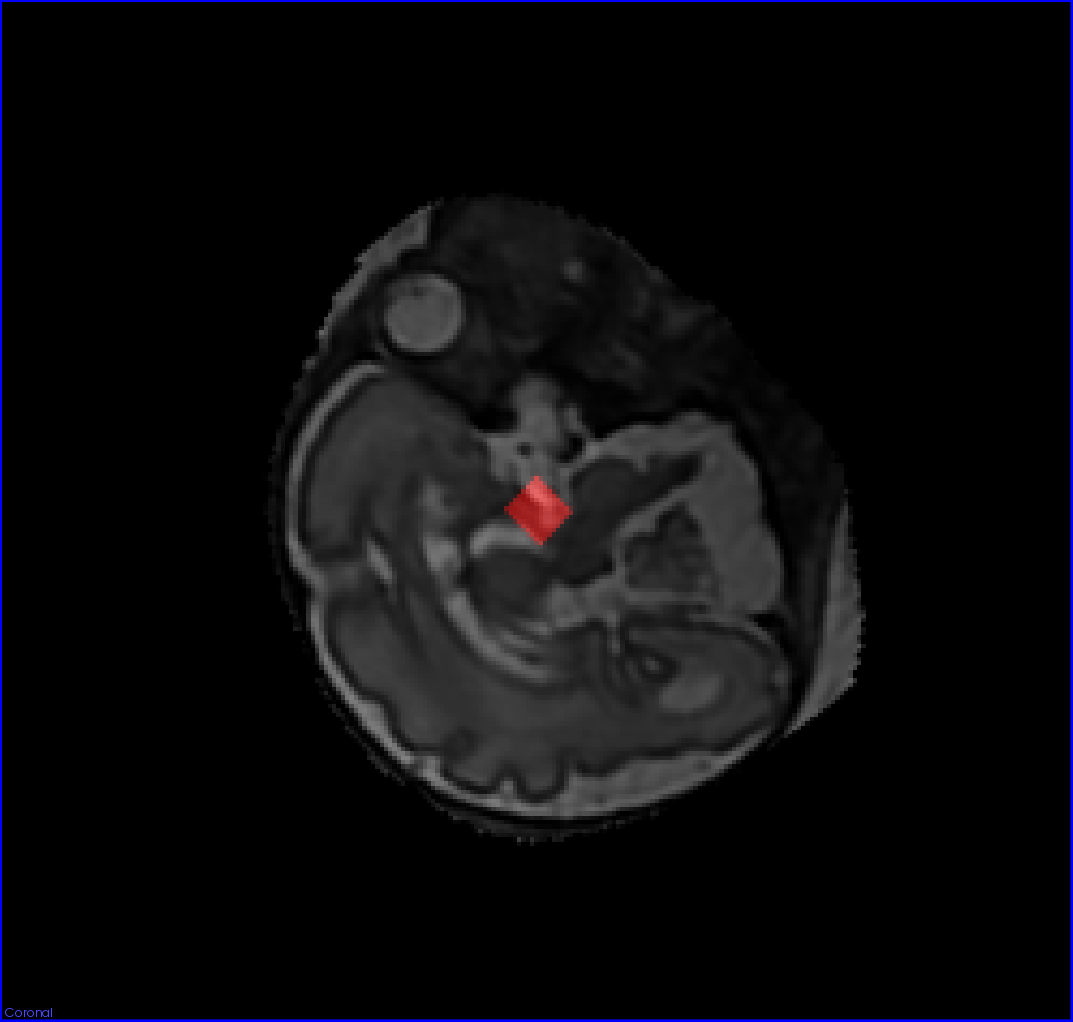
\includegraphics[width=\textwidth]{images/thresholding/results/cube_2d.png}
    \caption{Cube in 2D}
    \label{fig:thresholdingresultscube2d}
  \end{subfigure}%
  ~ %add desired spacing between images, e. g. ~, \quad, \qquad, \hfill etc.
    %(or a blank line to force the subfigure onto a new line)
  \begin{subfigure}[b]{0.32\textwidth}
    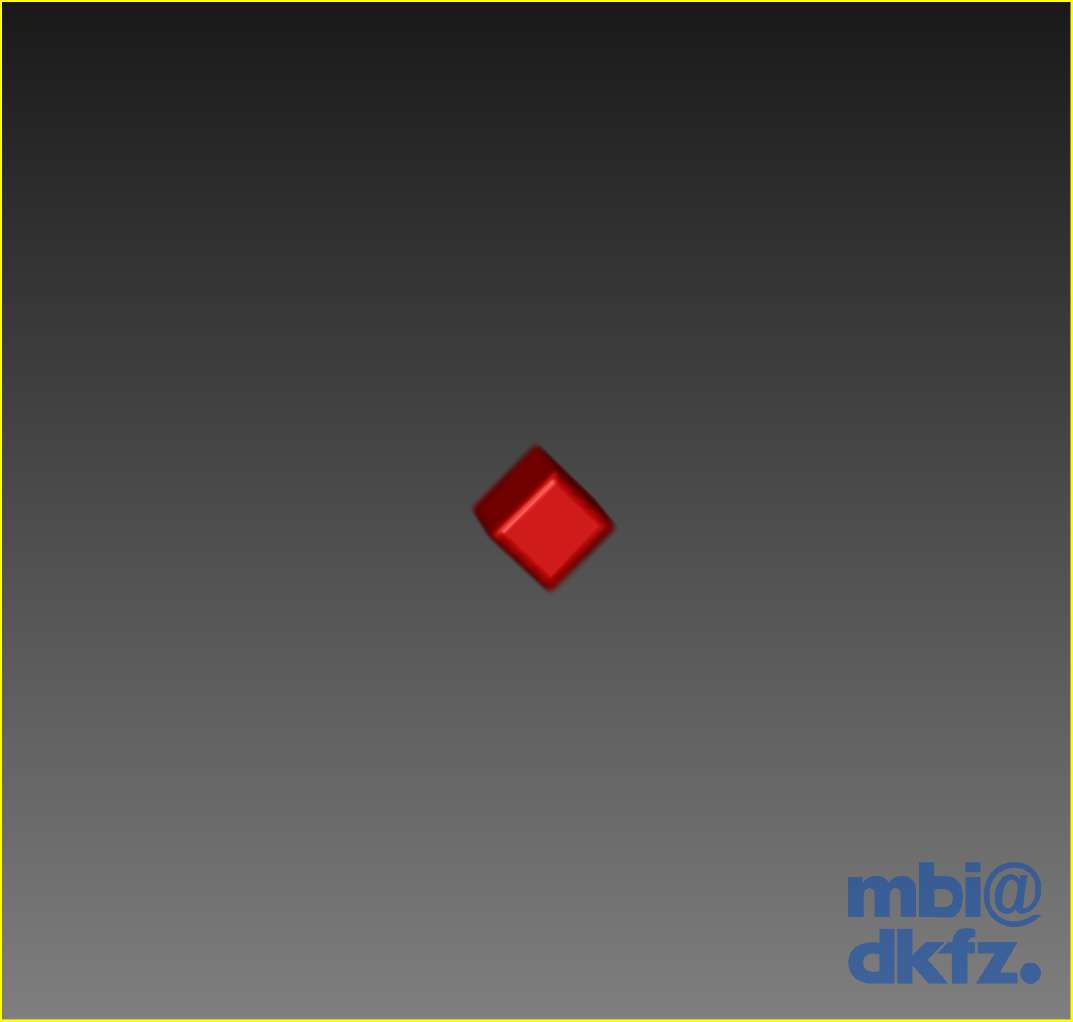
\includegraphics[width=\textwidth]{images/thresholding/results/cube_3d.png}
    \caption{Cube in 3D}
    \label{fig:thresholdingresultscube3d}
  \end{subfigure}
  ~ %add desired spacing between images, e. g. ~, \quad, \qquad, \hfill etc.
    %(or a blank line to force the subfigure onto a new line)
  \begin{subfigure}[b]{0.32\textwidth}
    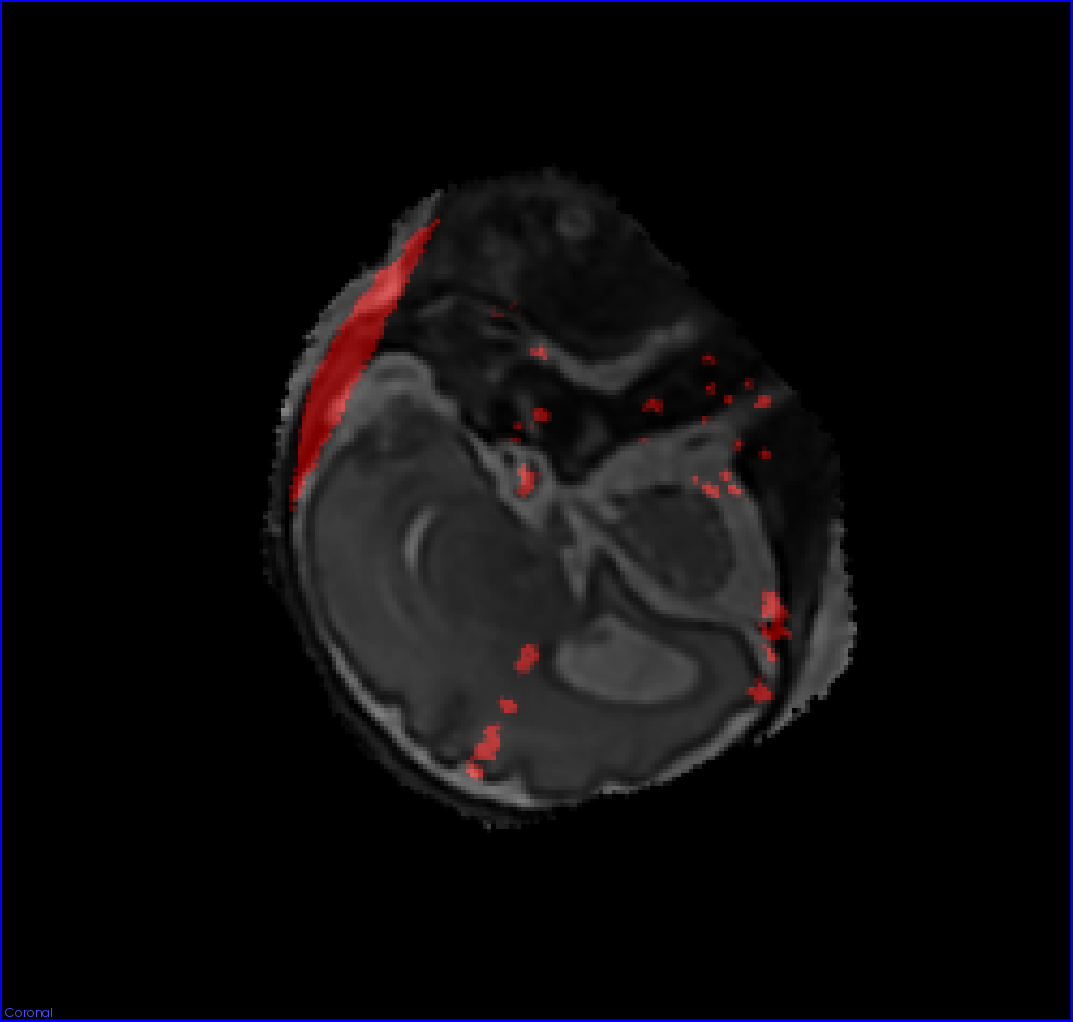
\includegraphics[width=\textwidth]{images/thresholding/results/scan_2d.png}
    \caption{Scan in 2D}
    \label{fig:thresholdingresultsscan2d}
  \end{subfigure}%
  ~ %add desired spacing between images, e. g. ~, \quad, \qquad, \hfill etc.
    %(or a blank line to force the subfigure onto a new line)
  \begin{subfigure}[b]{0.32\textwidth}
    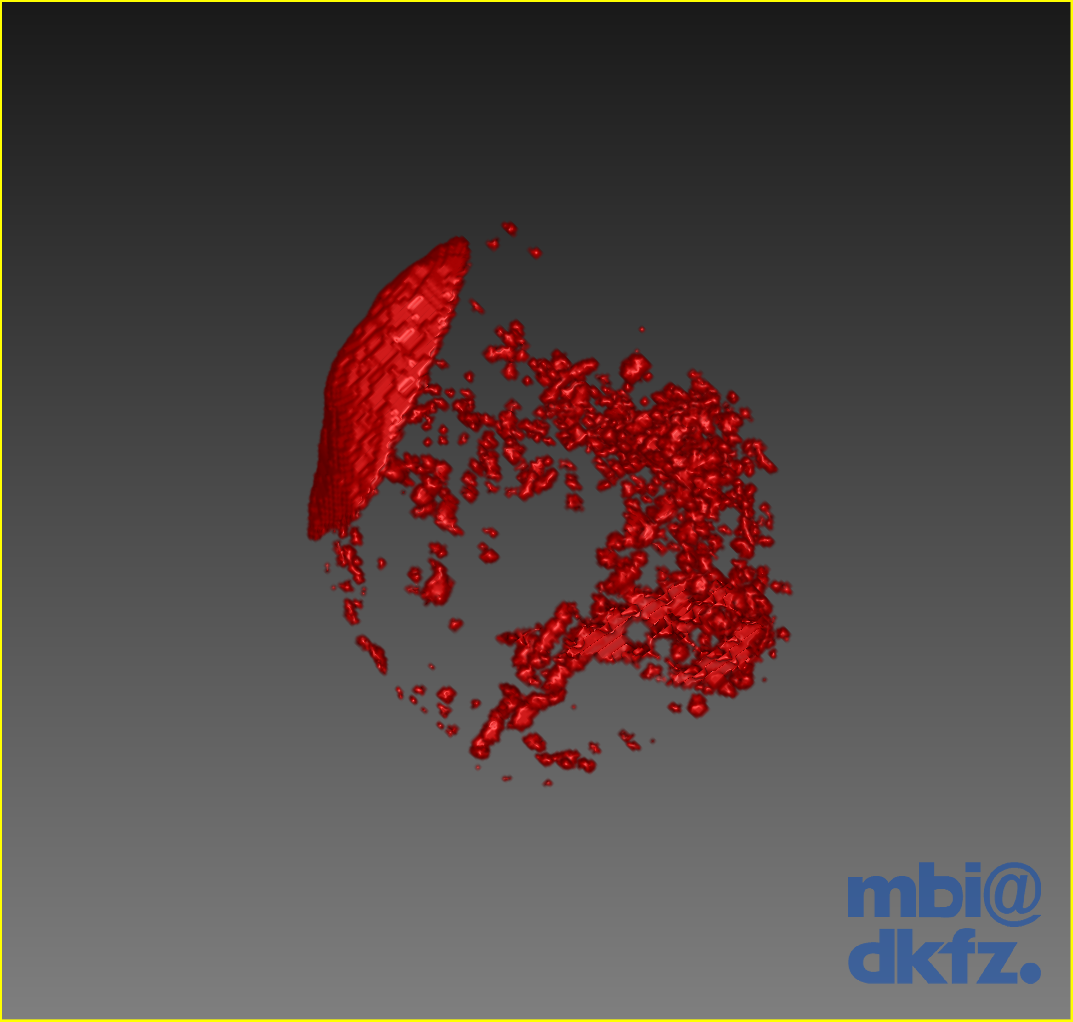
\includegraphics[width=\textwidth]{images/thresholding/results/scan_3d.png}
    \caption{Scan in 3D}
    \label{fig:thresholdingresultsscan3d}
  \end{subfigure}
  % \caption{Opacity Transfer Functions. Opacity of 0 is transparent, 1 is opaque.}\label{fig:thresholdingvariation1problem}
\end{figure}

\newpage
\section{Uncertainty Surface}\label{section:uncertaintysurface}

\newpage
\section{Next Scan Plane}\label{section:nextscanplane}

\newpage
\chapter{Tool}

\newpage
\section{Scan Simulation}\label{section:simulatescan}

\newpage
\section{Reconstruction}\label{section:reconstruction}